% !TEX encoding = UTF-8 Unicode
%% bare_conf_compsoc.tex
%% V1.4b
%% 2015/08/26
%% by Michael Shell
%% See:
%% http://www.michaelshell.org/
%% for current contact information.
%%
%% This is a skeleton file demonstrating the use of IEEEtran.cls
%% (requires IEEEtran.cls version 1.8b or later) with an IEEE Computer
%% Society conference paper.
%%
%% Support sites:
%% http://www.michaelshell.org/tex/ieeetran/
%% http://www.ctan.org/pkg/ieeetran
%% and
%% http://www.ieee.org/

%%*************************************************************************
%% Legal Notice:
%% This code is offered as-is without any warranty either expressed or
%% implied; without even the implied warranty of MERCHANTABILITY or
%% FITNESS FOR A PARTICULAR PURPOSE! 
%% User assumes all risk.
%% In no event shall the IEEE or any contributor to this code be liable for
%% any damages or losses, including, but not limited to, incidental,
%% consequential, or any other damages, resulting from the use or misuse
%% of any information contained here.
%%
%% All comments are the opinions of their respective authors and are not
%% necessarily endorsed by the IEEE.
%%
%% This work is distributed under the LaTeX Project Public License (LPPL)
%% ( http://www.latex-project.org/ ) version 1.3, and may be freely used,t
%% distributed and modified. A copy of the LPPL, version 1.3, is included
%% in the base LaTeX documentation of all distributions of LaTeX released
%% 2003/12/01 or later.
%% Retain all contribution notices and credits.
%% ** Modified files should be clearly indicated as such, including  **
%% ** renaming them and changing author support contact information. **
%%*************************************************************************


% *** Authors should verify (and, if needed, correct) their LaTeX system  ***
% *** with the testflow diagnostic prior to trusting their LaTeX platform ***
% *** with production work. The IEEE's font choices and paper sizes can   ***
% *** trigger bugs that do not appear when using other class files.       ***                          ***
% The testflow support page is at:
% http://www.michaelshell.org/tex/testflow/



\documentclass[conference,compsoc]{IEEEtran}
% Some/most Computer Society conferences require the compsoc mode option,
% but others may want the standard conference format.
%
% If IEEEtran.cls has not been installed into the LaTeX system files,
% manually specify the path to it like:
% \documentclass[conference,compsoc]{../sty/IEEEtran}





% Some very useful LaTeX packages include:
% (uncomment the ones you want to load)


% *** MISC UTILITY PACKAGES ***
%
%\usepackage{ifpdf}
% Heiko Oberdiek's ifpdf.sty is very useful if you need conditional
% compilation based on whether the output is pdf or dvi.
% usage:
% \ifpdf
%   % pdf code
% \else
%   % dvi code
% \fi
% The latest version of ifpdf.sty can be obtained from:
% http://www.ctan.org/pkg/ifpdf
% Also, note that IEEEtran.cls V1.7 and later provides a builtin
% \ifCLASSINFOpdf conditional that works the same way.
% When switching from latex to pdflatex and vice-versa, the compiler may
% have to be run twice to clear warning/error messages.


\usepackage[utf8]{inputenc}
\usepackage[portuguese]{babel}

\usepackage{url}
\usepackage{hyperref} 
\usepackage{graphicx}
\usepackage{fancyref}
\usepackage{amsmath}
\usepackage{multirow}
\usepackage{fancyhdr}
\pagestyle{fancy}

\usepackage{listings,mdframed}


\lstset{
	language=c,
	keywordstyle=\bfseries\ttfamily\color[rgb]{0,0,1},
	identifierstyle=\ttfamily,
	commentstyle=\color[rgb]{0.133,0.545,0.133},
	stringstyle=\ttfamily\color[rgb]{0.627,0.126,0.941},
	showstringspaces=false,
	basicstyle=\tiny,
numberstyle=\tiny,
numbers=right,
	stepnumber=1,
	numbersep=10pt,
	tabsize=1,
	breaklines=true,
	prebreak = \raisebox{0ex}[0ex][0ex]{\ensuremath{\hookleftarrow}},
	breakatwhitespace=false,
	aboveskip={1.5\baselineskip},
  columns=fixed,
  upquote=true,
  extendedchars=true,
 frame=single,
 inputencoding=utf8,
    literate={á}{{\'a}}1 {ã}{{\~a}}1 {â}{{\~a}}1 {é}{{\'e}}1 {ê}{{\'e}}1 {ç}{{\'c}}1 {ú}{{\'u}}1 {ó}{{\'o}}1 {í}{{\'i}}1,
 %backgroundcolor=\color{lbcolor},
}

% *** CITATION PACKAGES ***
%
\ifCLASSOPTIONcompsoc
  % IEEE Computer Society needs nocompress option
  % requires cite.sty v4.0 or later (November 2003)
  \usepackage[nocompress]{cite}
\else
  % normal IEEE
  \usepackage{cite}
\fi
% cite.sty was written by Donald Arseneau
% V1.6 and later of IEEEtran pre-defines the format of the cite.sty package
% \cite{} output to follow that of the IEEE. Loading the cite package will
% result in citation numbers being automatically sorted and properly
% "compressed/ranged". e.g., [1], [9], [2], [7], [5], [6] without using
% cite.sty will become [1], [2], [5]--[7], [9] using cite.sty. cite.sty's
% \cite will automatically add leading space, if needed. Use cite.sty's
% noadjust option (cite.sty V3.8 and later) if you want to turn this off
% such as if a citation ever needs to be enclosed in parenthesis.
% cite.sty is already installed on most LaTeX systems. Be sure and use
% version 5.0 (2009-03-20) and later if using hyperref.sty.
% The latest version can be obtained at:
% http://www.ctan.org/pkg/cite
% The documentation is contained in the cite.sty file itself.
%
% Note that some packages require special options to format as the Computer
% Society requires. In particular, Computer Society  papers do not use
% compressed citation ranges as is done in typical IEEE papers
% (e.g., [1]-[4]). Instead, they list every citation separately in order
% (e.g., [1], [2], [3], [4]). To get the latter we need to load the cite
% package with the nocompress option which is supported by cite.sty v4.0
% and later.





% *** GRAPHICS RELATED PACKAGES ***
%
\ifCLASSINFOpdf
  % \usepackage[pdftex]{graphicx}
  % declare the path(s) where your graphic files are
  % \graphicspath{{../pdf/}{../jpeg/}}
  % and their extensions so you won't have to specify these with
  % every instance of \includegraphics
  % \DeclareGraphicsExtensions{.pdf,.jpeg,.png}
\else
  % or other class option (dvipsone, dvipdf, if not using dvips). graphicx
  % will default to the driver specified in the system graphics.cfg if no
  % driver is specified.
  % \usepackage[dvips]{graphicx}
  % declare the path(s) where your graphic files are
  % \graphicspath{{../eps/}}
  % and their extensions so you won't have to specify these with
  % every instance of \includegraphics
  % \DeclareGraphicsExtensions{.eps}
\fi
% graphicx was written by David Carlisle and Sebastian Rahtz. It is
% required if you want graphics, photos, etc. graphicx.sty is already
% installed on most LaTeX systems. The latest version and documentation
% can be obtained at: 
% http://www.ctan.org/pkg/graphicx
% Another good source of documentation is "Using Imported Graphics in
% LaTeX2e" by Keith Reckdahl which can be found at:
% http://www.ctan.org/pkg/epslatex
%
% latex, and pdflatex in dvi mode, support graphics in encapsulated
% postscript (.eps) format. pdflatex in pdf mode supports graphics
% in .pdf, .jpeg, .png and .mps (metapost) formats. Users should ensure
% that all non-photo figures use a vector format (.eps, .pdf, .mps) and
% not a bitmapped formats (.jpeg, .png). The IEEE frowns on bitmapped formats
% which can result in "jaggedy"/blurry rendering of lines and letters as
% well as large increases in file sizes.
%
% You can find documentation about the pdfTeX application at:
% http://www.tug.org/applications/pdftex





% *** MATH PACKAGES ***
%
%\usepackage{amsmath}
% A popular package from the American Mathematical Society that provides
% many useful and powerful commands for dealing with mathematics.
%
% Note that the amsmath package sets \interdisplaylinepenalty to 10000
% thus preventing page breaks from occurring within multiline equations. Use:
%\interdisplaylinepenalty=2500
% after loading amsmath to restore such page breaks as IEEEtran.cls normally
% does. amsmath.sty is already installed on most LaTeX systems. The latest
% version and documentation can be obtained at:
% http://www.ctan.org/pkg/amsmath





% *** SPECIALIZED LIST PACKAGES ***
%
%\usepackage{algorithmic}
% algorithmic.sty was written by Peter Williams and Rogerio Brito.
% This package provides an algorithmic environment fo describing algorithms.
% You can use the algorithmic environment in-text or within a figure
% environment to provide for a floating algorithm. Do NOT use the algorithm
% floating environment provided by algorithm.sty (by the same authors) or
% algorithm2e.sty (by Christophe Fiorio) as the IEEE does not use dedicated
% algorithm float types and packages that provide these will not provide
% correct IEEE style captions. The latest version and documentation of
% algorithmic.sty can be obtained at:
% http://www.ctan.org/pkg/algorithms
% Also of interest may be the (relatively newer and more customizable)
% algorithmicx.sty package by Szasz Janos:
% http://www.ctan.org/pkg/algorithmicx




% *** ALIGNMENT PACKAGES ***
%
%\usepackage{array}
% Frank Mittelbach's and David Carlisle's array.sty patches and improves
% the standard LaTeX2e array and tabular environments to provide better
% appearance and additional user controls. As the default LaTeX2e table
% generation code is lacking to the point of almost being broken with
% respect to the quality of the end results, all users are strongly
% advised to use an enhanced (at the very least that provided by array.sty)
% set of table tools. array.sty is already installed on most systems. The
% latest version and documentation can be obtained at:
% http://www.ctan.org/pkg/array


% IEEEtran contains the IEEEeqnarray family of commands that can be used to
% generate multiline equations as well as matrices, tables, etc., of high
% quality.




% *** SUBFIGURE PACKAGES ***
%\ifCLASSOPTIONcompsoc
%  \usepackage[caption=false,font=footnotesize,labelfont=sf,textfont=sf]{subfig}
%\else
%  \usepackage[caption=false,font=footnotesize]{subfig}
%\fi
% subfig.sty, written by Steven Douglas Cochran, is the modern replacement
% for subfigure.sty, the latter of which is no longer maintained and is
% incompatible with some LaTeX packages including fixltx2e. However,
% subfig.sty requires and automatically loads Axel Sommerfeldt's caption.sty
% which will override IEEEtran.cls' handling of captions and this will result
% in non-IEEE style figure/table captions. To prevent this problem, be sure
% and invoke subfig.sty's "caption=false" package option (available since
% subfig.sty version 1.3, 2005/06/28) as this is will preserve IEEEtran.cls
% handling of captions.
% Note that the Computer Society format requires a sans serif font rather
% than the serif font used in traditional IEEE formatting and thus the need
% to invoke different subfig.sty package options depending on whether
% compsoc mode has been enabled.
%
% The latest version and documentation of subfig.sty can be obtained at:
% http://www.ctan.org/pkg/subfig




% *** FLOAT PACKAGES ***
%
%\usepackage{fixltx2e}
% fixltx2e, the successor to the earlier fix2col.sty, was written by
% Frank Mittelbach and David Carlisle. This package corrects a few problems
% in the LaTeX2e kernel, the most notable of which is that in current
% LaTeX2e releases, the ordering of single and double column floats is not
% guaranteed to be preserved. Thus, an unpatched LaTeX2e can allow a
% single column figure to be placed prior to an earlier double column
% figure.
% Be aware that LaTeX2e kernels dated 2015 and later have fixltx2e.sty's
% corrections already built into the system in which case a warning will
% be issued if an attempt is made to load fixltx2e.sty as it is no longer
% needed.
% The latest version and documentation can be found at:
% http://www.ctan.org/pkg/fixltx2e


%\usepackage{stfloats}
% stfloats.sty was written by Sigitas Tolusis. This package gives LaTeX2e
% the ability to do double column floats at the bottom of the page as well
% as the top. (e.g., "\begin{figure*}[!b]" is not normally possible in
% LaTeX2e). It also provides a command:
%\fnbelowfloat
% to enable the placement of footnotes below bottom floats (the standard
% LaTeX2e kernel puts them above bottom floats). This is an invasive package
% which rewrites many portions of the LaTeX2e float routines. It may not work
% with other packages that modify the LaTeX2e float routines. The latest
% version and documentation can be obtained at:
% http://www.ctan.org/pkg/stfloats
% Do not use the stfloats baselinefloat ability as the IEEE does not allow
% \baselineskip to stretch. Authors submitting work to the IEEE should note
% that the IEEE rarely uses double column equations and that authors should try
% to avoid such use. Do not be tempted to use the cuted.sty or midfloat.sty
% packages (also by Sigitas Tolusis) as the IEEE does not format its papers in
% such ways.
% Do not attempt to use stfloats with fixltx2e as they are incompatible.
% Instead, use Morten Hogholm'a dblfloatfix which combines the features
% of both fixltx2e and stfloats:
%
% \usepackage{dblfloatfix}
% The latest version can be found at:
% http://www.ctan.org/pkg/dblfloatfix




% *** PDF, URL AND HYPERLINK PACKAGES ***
%
%\usepackage{url}
% url.sty was written by Donald Arseneau. It provides better support for
% handling and breaking URLs. url.sty is already installed on most LaTeX
% systems. The latest version and documentation can be obtained at:
% http://www.ctan.org/pkg/url
% Basically, \url{my_url_here}.




% *** Do not adjust lengths that control margins, column widths, etc. ***
% *** Do not use packages that alter fonts (such as pslatex).         ***
% There should be no need to do such things with IEEEtran.cls V1.6 and later.
% (Unless specifically asked to do so by the journal or conference you plan
% to submit to, of course. )


% correct bad hyphenation here
\hyphenation{op-tical net-works semi-conduc-tor}


\begin{document}
%
% paper title
% Titles are generally capitalized except for words such as a, an, and, as,
% at, but, by, for, in, nor, of, on, or, the, to and up, which are usually
% not capitalized unless they are the first or last word of the title.
% Linebreaks \\ can be used within to get better formatting as desired.
% Do not put math or special symbols in the title.
\title{\textit{Profiling} de \textit{Software/Hardware} com \textit{Perf}}


% author names and affiliations
% use a multiple column layout for up to three different
% affiliations
\author{\IEEEauthorblockN{Sérgio Caldas}
\IEEEauthorblockA{Universidade do Minho\\Escola de Engenharia\\Departamento de Informática\\
Email: a57779@alunos.uminho.pt}}

% conference papers do not typically use \thanks and this command
% is locked out in conference mode. If really needed, such as for
% the acknowledgment of grants, issue a \IEEEoverridecommandlockouts
% after \documentclass

% for over three affiliations, or if they all won't fit within the width
% of the page (and note that there is less available width in this regard for
% compsoc conferences compared to traditional conferences), use this
% alternative format:
% 
%\author{\IEEEauthorblockN{Michael Shell\IEEEauthorrefmark{1},
%Homer Simpson\IEEEauthorrefmark{2},
%James Kirk\IEEEauthorrefmark{3}, 
%Montgomery Scott\IEEEauthorrefmark{3} and
%Eldon Tyrell\IEEEauthorrefmark{4}}
%\IEEEauthorblockA{\IEEEauthorrefmark{1}School of Electrical and Computer Engineering\\
%Georgia Institute of Technology,
%Atlanta, Georgia 30332--0250\\ Email: see http://www.michaelshell.org/contact.html}
%\IEEEauthorblockA{\IEEEauthorrefmark{2}Twentieth Century Fox, Springfield, USA\\
%Email: homer@thesimpsons.com}
%\IEEEauthorblockA{\IEEEauthorrefmark{3}Starfleet Academy, San Francisco, California 96678-2391\\
%Telephone: (800) 555--1212, Fax: (888) 555--1212}
%\IEEEauthorblockA{\IEEEauthorrefmark{4}Tyrell Inc., 123 Replicant Street, Los Angeles, California 90210--4321}}




% use for special paper notices
%\IEEEspecialpapernotice{(Invited Paper)}




% make the title area
\maketitle
\tableofcontents
\vspace{0.5cm}
% As a general rule, do not put math, special symbols or citations
% in the abstract
\begin{abstract}
Este artigo, representa o relatório do trabalho prático nº5, desenvolvido no âmbito da disciplina de Engenharia de Sistemas de Computação (ESC), inserida no perfil de Computação Paralela e Distribuída (CPD) do curso de Engenharia Informática. O objetivo deste trabalho é seguirmos um tutorial\cite{tutorial} providenciado pelo professor, com o intuito de iniciarmos e praticarmos a utilização da ferramenta \textit{Perf}. 

Para a execução deste trabalho, para além do tutorial, também nos foi facultado um código (\textit{naive.c}), este código efectua a multiplicação de matrizes. Com este código e juntamente com a ferramenta \textit{Perf}, procedi ao \textit{profiling} do mesmo, utilizando diferentes comandos desta ferramenta. Com estes comandos é possível fazermos \textit{profiling}, quer com contadores de \textit{software}, quer com contadores de \textit{hardware} 

\end{abstract}

% no keywords




% For peer review papers, you can put extra information on the cover
% page as needed:
% \ifCLASSOPTIONpeerreview
% \begin{center} \bfseries EDICS Category: 3-BBND \end{center}
% \fi
%
% For peerreview papers, this IEEEtran command inserts a page break and
% creates the second title. It will be ignored for other modes.
\IEEEpeerreviewmaketitle



\section{Introdução}

Este trabalho está dividido em 3 partes, assim como o tutorial providênciado, a primeira parte diz respeito à deteção de \textit{hot spots} da execução da aplicação produzida pelo código facultado, esta primeira parte, cobre os comandos e opções básicas da ferramenta \textit{Perf} assim como os seus eventos de desempenho de software mais básicos. 

A segunda parte introduz os eventos de desempenho de \textit{hardware}, sendo que o tutorial faz uma demonstração de como realizar medições dos eventos de \textit{hardware} em torno de toda a aplicação. Nesta segunda parte para além do código referido atrás é também utilizada uma versão optimizada desse mesmo código (\textit{interchange.c}).

Na terceira e ultima parte deste  tutorial, utilizo amostras de eventos de desempenho de \textit{hardware} para identificar e analisar \textit{"hotspots"} nos programas que são testados. Nesta parte são testados dois programas o \textit{naive\_large}, que corresponde ao programa \textit{naive} referido atrás mas com uma maior dimensão to tamanho das matrizes e o programa \textit{interchange\_large} que corresponde a uma versão com uma maior dimensão do tamanho das matizes para o programa optimizado referido atrás.

Por fim, neste trabalho, também procedemos a geração de \textit{FlameGraphs}, para cada uma das aplicações. Estes gráficos foram obtidos através dos dados recolhidos com o \textit{perf} e tratados com \textit{scripts} específicas, posteriormente.

Neste relatório, apresento todos os meus resultados obtidos na realização e no acompanhamento do tutorial referido, bem como a análise desses mesmos resultados.

\section{\textit{Perf}}
O \textit{Perf} é uma ferramenta de análise de \textit{performance} desenvolvida para \textit{LINUX}, esta ferramenta é acessível através da linha de comandos e fornece uma gama de sub-comandos bem como uma basta gama de contadores, tanto de \textit{hardware} como de \textit{software}. Estes comandos permitem fazer uma análise estatística de todo o sistema, quer ao nível do \textit{Kernel} quer ao nível do utilizador.

Esta ferramenta para além dos referidos contadores, providência também \textit{Tracepoints} e provas dinâmicas como por exemplo \textit{kprobes} ou \textit{uprobes}.

O \textit{Perf} apresenta um conjunto de comandos principais (os mais utilizados), esses comandos encontam-se listados e explicados em baixo:

\begin{itemize}
	\item \textit{perf stat} - este comando permite fazer uma recolha estatística dos principais eventos do \textit{Perf}, se quisermos selecioanar apenas um sub-conjunto desses principais eventos apenas temos de adicionar ao comando a \textit{flag} -e juntamente com o nome dos eventos desejados, como por exemplo \textit{perf stat -e cpu-clock}. O comando referido é um comando mais leve em relação aos restantes comandos do \textit{Perf}.
	\item \textit{perf record} - este comando faz uma captura/gravação dos dados dos contadores especificados no ficheiro \textit{perf.data}, para posteriormente serem tratados pelo comando \textit{perf report}. O comando \textit{perf record} à semelhança do comando do ponto anterior também permite selecionarmos quais os eventos que queremos recolher informação, para isso só temos de adicionar ao comando a \textit{flag} -e juntamente com o nome dos eventos desejados, como por exemplo \textit{perf record -e cpu-clock,faults}.
	\item \textit{perf report} - com este comando é possível consultarmos e analisarmos os dados guardados no ficheiro \textit{perf.data}. Este comando à semelhança dos outros também permite uma gama de opções/\textit{flags}. Para a seleção da \textit{interface do utilizador} podemos usar os seguintes opções:
	\begin{itemize}
		\item \textit{- -tui}, esta opção permite selecionar uma \textit{interface} baseada na linha de comandos. Esta opção suporta uma navegação \textit{interativa}.
		\item \textit{- -stdio}, esta opção imprime o \textit{output} do \textit{profile} capturado no \textit{standard output}.
		\item \textit{- -gtk} esta opção seleciona a \textit{GTK interface}. 
	\end{itemize}
\end{itemize}

Para além dos comandos atrás referidos, o \textit{Perf} ainda contem um conjunto de contadores pré-definidos tais como:
\begin{itemize}
	\item cpu-clock
	\item task-clock
	\item page-faults OR faults
	\item context-switches OR cs
	\item cpu-migrations OR migrations
	\item minor-faults
	\item major-faults
	\item alignment-faults
	\item emulation-faults
\end{itemize}

A versão do \textit{Perf} utilizada na realização deste trabalho é a versão 4.0.0.

\section{Caracterização do Ambiente de Testes}

A máquina utilizada para se realizar este trabalho, foi um nó do \textit{Cluster search} mais especificamente o nó \textit{431}. Na tabela \ref{t:431} encontra-se a especificação desse mesmo nó.

\begin{table}[h!]
\centering
\begin{tabular}{ | l | c | }
\hline
System & Máquina 431\\ 
\hline 
\hline
\# CPUs & 2\\ 
\hline
CPU & Intel\textsuperscript{\textregistered} Xeon\textsuperscript{\textregistered} X5650\\
\hline 
Architecture & Nehalem\\ 
\hline 
\# Cores per CPU & 6\\ 
\hline 
\# Threads per CPU & 12\\ 
\hline 
Clock Freq. & 2.66 GHz\\ 
\hline 
\hline 
L1 Cache & 192 KB \newline 32 KB por core\\ 
\hline 
L2 Cache & 1536 KB \newline 256 KB por core\\ 
\hline 
L3 Cache & 12 MB\\ 
\hline 
\hline 
Inst. Set Ext. & SSE4.2 e AVX\\
 \hline 
\#Memory Channels & 3\\ 
\hline 
Memory BW & 32 GB/s\\
\hline
\end{tabular}
\caption{Caracterização da Máquina 431}
\label{t:431}
\end{table}

Para a compilação dos programas referidos anteriormente foi carregado neste nó o modulo com o gnu/4.9.0, para além desta versão todos os programas foram compilados com a \textit{flag} -O2 -ggdb -g -c.

\section{Parte 1 - Procura dos pontos quentes de uma aplicação em execução}

A primeira parte deste trabalho, foca-se essencialmente na procura de pontos quentes de uma aplicação em execução, para isso iniciei o tutorial exatamente pela sua primeira parte. 

Inicialmente comecei por testar alguns comandos básicos do \textit{Perf}, comandos como,

\begin{lstlisting}
perf - -help
\end{lstlisting}

este comando apresenta uma lista com todos os comandos todos os comandos mais utilizados do \textit{Perf} como pode ser consultado em baixo.

\begin{lstlisting}
 The most commonly used perf commands are:
   annotate        Read perf.data (created by perf record) and display annotated code
   archive         Create archive with object files with build-ids found in perf.data file
   bench           General framework for benchmark suites
   buildid-cache   Manage build-id cache.
   buildid-list    List the buildids in a perf.data file
   diff            Read perf.data files and display the differential profile
   evlist          List the event names in a perf.data file
   inject          Filter to augment the events stream with additional information
   kmem            Tool to trace/measure kernel memory(slab) properties
   kvm             Tool to trace/measure kvm guest os
   list            List all symbolic event types
   lock            Analyze lock events
   mem             Profile memory accesses
   record          Run a command and record its profile into perf.data
   report          Read perf.data (created by perf record) and display the profile
   sched           Tool to trace/measure scheduler properties (latencies)
   script          Read perf.data (created by perf record) and display trace output
   stat            Run a command and gather performance counter statistics
   test            Runs sanity tests.
   timechart       Tool to visualize total system behavior during a workload
   top             System profiling tool.
   trace           strace inspired tool
   probe           Define new dynamic tracepoints
\end{lstlisting}

Se quisermos obter mais informação relativamente aos comandos apresentados em cima basta-nos executar o seguinte comando:

\begin{lstlisting}
perf help COMMAND
\end{lstlisting}

ou

\begin{lstlisting}
perf COMMAND - -help
\end{lstlisting}

Como foi referido anteriormente, o \textit{Perf} suporta, quer eventos de \textit{Software} quer eventos de \textit{Hardware}. Para termos acesso à lista de eventos disponíveis na máquina, só temos de executar o comando em baixo exemplificado. 

\begin{lstlisting}
perf list
\end{lstlisting}

Ao executarmos esse comando é-nos apresentado uma lista com todos os eventos disponíveis na máquina. Como podemos ver na lista em baixo.

\begin{lstlisting}
  cpu-cycles OR cycles                               [Hardware event]
  instructions                                       [Hardware event]
  cache-references                                   [Hardware event]
  cache-misses                                       [Hardware event]
  branch-instructions OR branches                    [Hardware event]
  branch-misses                                      [Hardware event]
  stalled-cycles-frontend OR idle-cycles-frontend    [Hardware event]
  stalled-cycles-backend OR idle-cycles-backend      [Hardware event]

  cpu-clock                                          [Software event]
  task-clock                                         [Software event]
  page-faults OR faults                              [Software event]
  context-switches OR cs                             [Software event]
  cpu-migrations OR migrations                       [Software event]
  minor-faults                                       [Software event]
  major-faults                                       [Software event]
  alignment-faults                                   [Software event]
  emulation-faults                                   [Software event]

  L1-dcache-loads                                    [Hardware cache event]
  L1-dcache-load-misses                              [Hardware cache event]
  L1-dcache-stores                                   [Hardware cache event]
  L1-dcache-store-misses                             [Hardware cache event]
  L1-dcache-prefetches                               [Hardware cache event]
  L1-dcache-prefetch-misses                          [Hardware cache event]
  L1-icache-loads                                    [Hardware cache event]
  L1-icache-load-misses                              [Hardware cache event]
  LLC-loads                                          [Hardware cache event]
  LLC-load-misses                                    [Hardware cache event]
  LLC-stores                                         [Hardware cache event]
  LLC-store-misses                                   [Hardware cache event]
  LLC-prefetches                                     [Hardware cache event]
  LLC-prefetch-misses                                [Hardware cache event]
  dTLB-loads                                         [Hardware cache event]
  dTLB-load-misses                                   [Hardware cache event]
  dTLB-stores                                        [Hardware cache event]
  dTLB-store-misses                                  [Hardware cache event]
  iTLB-loads                                         [Hardware cache event]
  iTLB-load-misses                                   [Hardware cache event]
  branch-loads                                       [Hardware cache event]
  branch-load-misses                                 [Hardware cache event]
\end{lstlisting}

\subsection{Tempo de Execução e Contagem de Eventos}

Depois de uma familiarização mais básica com a ferramenta \textit{Perf}, passei então à análise da aplicação em questão. De referir mais uma vez que o código utilizado nesta primeira parte do tutorial foi o código \textit{naive.c}.

Para se fazer uma boa análise da aplicação em execução, temos de ter uma referência, isto é, uma base por onde nos podemos guiar. Então o primeiro paço deste tutorial, é fazer uma recolha estatística da aplicação em execução, para isso o evento \textit{cpu-clock} é o evento que precisamos, este evento dá-nos o número de \textit{cpu-clock} em milissegundos, bem como o tempo gasto na execução. O comando utilizado para fazer esta recolha estatística foi o seguinte:

\begin{lstlisting}
perf stat -e cpu-clock ./naive
\end{lstlisting} 

sendo que o seu \textit{output} foi o seguinte:

\begin{lstlisting}
 Performance counter stats for './naive':

        185.696104      cpu-clock (msec)                                            

       0.187093191 seconds time elapsed
\end{lstlisting} 

Para além do evento \textit{cpu-clock} podemos medir mais do que um evento, para isso só temos de executar o comando com a \textit{flag} -e juntamente com o sub-conjunto de eventos desejados. Como mostra o exemplo seguinte:


\begin{lstlisting}
perf stat -e cpu-clock,faults ./naive
\end{lstlisting}

O \textit{output} do comando em cima exemplificado foi:

\begin{lstlisting}
 Performance counter stats for './naive':

        182.586308      cpu-clock (msec)                                            
               845      faults                                                      

       0.184159812 seconds time elapsed
\end{lstlisting}

As regiões do código que gastam a maior parte do tempo de execução, são chamadas de \textit{hotspots}, estas regiões são as melhores regiões para se fazer alterações no código, de forma a optimiza-lo, pois com um pequeno esforço podemos ter grandes ganhos.

Depois de medirmos os \textit{cpu-clocks} e as \textit{page-faults}, perguntámos-nos se estas eventos indicam um problema de desempenho ou não?! O número 845 de \textit{page-faults} é demasiado?! Para respondermos a estas questões é necessário termos um conhecimento aprofundado da estrutura do código bem como das suas estruturas de dados. Pelo menos temos de saber se a aplicação é \textit{Memory Bound} ou  \textit{CPU Bound}, isto é se perde demasiado tempo nos acessos à memória ou se efectua demasiado trabalho computacional respetivamente. 

Com o \textit{Perf} podemos fazer um profiling mais detalhado sobre a aplicação de forma a identificarmos esses problemas, para posteriormente serem optimizados e por fim efectuar novas medições de forma a serem comparadas com as medições que foram feitas no inicio deste tutorial. Só depois dessa comparação e dessa nova análise é que saberemos se tivemos algum \textit{speed-up} ou não.

\subsection{Procura de \textit{Hotsposts}}

Com a ajuda do \textit{Perf} é possível localizarmos \textit{hotspots} para isso temos de fazer um profiling da aplicação em questão, para isso executamos o comando \textit{perf record} que faz uma recolha de dados de perfil e guarda no ficheiro \textit{perf.data}. O comando executado para se fazer esta recolha foi o seguinte comando:

\begin{lstlisting}
perf record -e cpu-clock,faults ./naive
\end{lstlisting}

Neste caso especifico o \textit{Perf} faz uma recolha de dados de perfil para dois eventos: \textit{cpu-clock} e \textit{page-faults}. Depois destes dados serem recolhidos, estes são tratados com o comando \textit{perf report} este comando mostra-nos toda a informação guardada no ficheiro \textit{perf.data}. O comando utilizado para a análise dos dados contidos no ficheiro \textit{perf.data} foi o seguinte:

\begin{lstlisting}
perf report --stdio --sort comm,dso
\end{lstlisting}

sendo que o seu \textit{output} foi:

\begin{lstlisting}
# ========
# captured on: Tue May 24 00:12:26 2016
# hostname : compute-431-9.local
# os release : 2.6.32-279.14.1.el6.x86_64
# perf version : 4.0.0
# arch : x86_64
# nrcpus online : 24
# nrcpus avail : 24
# cpudesc : Intel(R) Xeon(R) CPU E5649 @ 2.53GHz
# cpuid : GenuineIntel,6,44,2
# total memory : 49551752 kB
# cmdline : /share/jade/SOFT/perf/perf record -e cpu-clock,faults ./naive 
# event : name = cpu-clock, type = 1, config = 0x0, config1 = 0x0, config2 = 0x0, excl_usr =
# event : name = faults, type = 1, config = 0x2, config1 = 0x0, config2 = 0x0, excl_usr = 0,
# HEADER_CPU_TOPOLOGY info available, use -I to display
# HEADER_NUMA_TOPOLOGY info available, use -I to display
# pmu mappings: cpu = 4, tracepoint = 2, software = 1
# ========
#
# Samples: 738  of event 'cpu-clock'
# Event count (approx.): 738
#
# Overhead  Command  Shared Object    
# ........  .......  .................
#
    97.29%  naive    naive            
     1.36%  naive    libc-2.12.so     
     1.22%  naive    [kernel.kallsyms]
     0.14%  naive    ld-2.12.so       


# Samples: 17  of event 'faults'
# Event count (approx.): 1245
#
# Overhead  Command  Shared Object    
# ........  .......  .................
#
    65.62%  naive    naive            
    33.98%  naive    ld-2.12.so       
     0.24%  naive    [kernel.kallsyms]
     0.16%  naive    libc-2.12.so 
\end{lstlisting}

Como podemos ver, pela a análise dos dados em cima apresentados,  podemos verificar que 97.29\% do tempo de execução é atribuída à aplicação \textit{naive}. Quanto ao número de \textit{page-faults} podemos verificar que 65.62\% é atribuída também á execução da aplicação \textit{naive}. Com esta informação sabemos que é a aplicação que está a ter um maior tempo de execução bem como um maior numero de \textit{page-faults}, contudo precisamos de ser mais minuciosos no nosso \textit{profiling}. Para isso executamos o comadno \textit{perf report} com a \textit{flag} --dsos. Com esta  \textit{flag} restringimos o \textit{output} ao objecto partilhado dinamicamente neste caso o programa \textit{naive}.

Como tal executamos o seguinte comando:

\begin{lstlisting}
perf report --stdio --dsos=naive,libc-2.13.so 
\end{lstlisting}

sendo que o seu \textit{output} é:

\begin{lstlisting}
# ========
# captured on: Tue May 24 00:12:26 2016
# hostname : compute-431-9.local
# os release : 2.6.32-279.14.1.el6.x86_64
# perf version : 4.0.0
# arch : x86_64
# nrcpus online : 24
# nrcpus avail : 24
# cpudesc : Intel(R) Xeon(R) CPU E5649 @ 2.53GHz
# cpuid : GenuineIntel,6,44,2
# total memory : 49551752 kB
# cmdline : /share/jade/SOFT/perf/perf record -e cpu-clock,faults ./naive 
# event : name = cpu-clock, type = 1, config = 0x0, config1 = 0x0, config2 = 0x0, excl_usr =
# event : name = faults, type = 1, config = 0x2, config1 = 0x0, config2 = 0x0, excl_usr = 0,
# HEADER_CPU_TOPOLOGY info available, use -I to display
# HEADER_NUMA_TOPOLOGY info available, use -I to display
# pmu mappings: cpu = 4, tracepoint = 2, software = 1
# ========
#
# Samples: 738  of event 'cpu-clock'
# Event count (approx.): 738
#
# Overhead  Command  Shared Object  Symbol                 
# ........  .......  .............  .......................
#
    95.66%  naive    naive          [.] multiply_matrices  
     1.49%  naive    naive          [.] initialize_matrices
     0.14%  naive    naive          [.] rand@plt           


# Samples: 17  of event 'faults'
# Event count (approx.): 1245
#
# Overhead  Command  Shared Object  Symbol                 
# ........  .......  .............  .......................
#
    65.62%  naive    naive          [.] initialize_matrices 
\end{lstlisting}

Ao analisarmos o \textit{output} em cima, já podemos ter uma ideia mais pormenorizada das funções onde é gasto a maior parte do tempo de execução e onde há um maior numero de \textit{page-faults} na aplicação. Como podemos ver, 95.66\% do tempo de execução da aplicação \textit{naive} é gasto na função \textit{multiply\_matrices}, e a função \textit{initialize\_matrices} é a função que apresenta um maior numero de \textit{page-faults} na aplicação. Com estes dados já estamos mais perto do \textit{hotspot} que procuramos, contudo ainda é possível aprofundarmos mais esta nossa pesquisa, para isso usamos o comando \textit{perf annotate} com a \textit{flag} --dsos e a \textit{flag} --symbol.
Para termos ainda uma analise mais detalhada, de forma a encontrarmos o \textit{hotspot}, executamos o seguinte comando:

\begin{lstlisting}
perf annotate --stdio --dsos=naive --symbol=multiply_matrices
\end{lstlisting}

sendo que o seu \textit{output} é o seguinte:

\begin{lstlisting}
 Percent |      Source code & Disassembly of naive for cpu-clock
----------------------------------------------------------------
         :
         :
         :
         :      Disassembly of section .text:
         :
         :      0000000000400810 <multiply_matrices>:
         :      multiply_matrices():
         :          }
         :        }
         :      }
         :       
         :      void multiply_matrices()
         :      {
    0.00 :        400810:       pxor   %xmm2,%xmm2
    0.00 :        400814:       mov    $0x7e97c0,%edi
    0.00 :        400819:       mov    %rdi,%r8
    0.00 :        40081c:       xor    %esi,%esi
    0.00 :        40081e:       sub    $0x7e97c0,%r8
    0.00 :        400825:       nopl   (%rax)
    0.00 :        400828:       lea    0x6f5580(%rsi),%rax
    0.00 :        40082f:       lea    0x7e97c0(%rsi),%rcx
    0.00 :        400836:       mov    %rdi,%rdx
    0.00 :        400839:       movaps %xmm2,%xmm1
    0.00 :        40083c:       nopl   0x0(%rax)
         :       
         :        for (i = 0 ; i < MSIZE ; i++) {
         :          for (j = 0 ; j < MSIZE ; j++) {
         :            float sum = 0.0 ;
         :            for (k = 0 ; k < MSIZE ; k++) {
         :              sum = sum + (matrix_a[i][k] * matrix_b[k][j]) ;
   24.65 :        400840:       movss  (%rdx),%xmm0
    0.28 :        400844:       add    $0x7d0,%rax
    0.00 :        40084a:       mulss  -0x7d0(%rax),%xmm0
   20.11 :        400852:       add    $0x4,%rdx
         :        int i, j, k ;
         :       
         :        for (i = 0 ; i < MSIZE ; i++) {
         :          for (j = 0 ; j < MSIZE ; j++) {
         :            float sum = 0.0 ;
         :            for (k = 0 ; k < MSIZE ; k++) {
   22.38 :        400856:       cmp    %rcx,%rax
         :              sum = sum + (matrix_a[i][k] * matrix_b[k][j]) ;
    0.00 :        400859:       addss  %xmm0,%xmm1
         :        int i, j, k ;
         :       
         :        for (i = 0 ; i < MSIZE ; i++) {
         :          for (j = 0 ; j < MSIZE ; j++) {
         :            float sum = 0.0 ;
         :            for (k = 0 ; k < MSIZE ; k++) {
   32.44 :        40085d:       jne    400840 <multiply_matrices+0x30>
         :              sum = sum + (matrix_a[i][k] * matrix_b[k][j]) ;
         :            }
         :            matrix_r[i][j] = sum ;
    0.00 :        40085f:       movss  %xmm1,0x601340(%r8,%rsi,1)
    0.14 :        400869:       add    $0x4,%rsi
         :      void multiply_matrices()
         :      {
         :        int i, j, k ;
         :       
         :        for (i = 0 ; i < MSIZE ; i++) {
         :          for (j = 0 ; j < MSIZE ; j++) {
    0.00 :        40086d:       cmp    $0x7d0,%rsi
    0.00 :        400874:       jne    400828 <multiply_matrices+0x18>
    0.00 :        400876:       add    $0x7d0,%rdi
         :       
         :      void multiply_matrices()
         :      {
         :        int i, j, k ;
         :       
         :        for (i = 0 ; i < MSIZE ; i++) {
    0.00 :        40087d:       cmp    $0x8dda00,%rdi
    0.00 :        400884:       jne    400819 <multiply_matrices+0x9>
    0.00 :        400886:       repz retq
\end{lstlisting}

Ao analisarmos o \textit{output} apresentado vemos qual a instrução que gasta um maior tempo de execução, com cerca de 32.44\%. A instrução em causa é a seguinte instrução:

\begin{lstlisting}
   32.44 :        40085d:       jne    400840 <multiply_matrices+0x30>
\end{lstlisting}

esta instrução corresponde ao seguinte excerto de código em \textit{C}:

\begin{lstlisting}
	sum = sum + (matrix_a[i][k] * matrix_b[k][j]) ;
\end{lstlisting}

Ou seja a maior parte do tempo gasto na execução da aplicação é gasta no calculo da multiplicação das duas matrizes e na adição do seu resultado à variável \textit{sum}. Com isto encontramos o \textit{hotspot}, sendo que o a parte mais \textit{hottest} da função \textit{multiply\_matrices} é o ciclo mais interno. Este ciclo corresponde ao excerto de código em \textit{C} apresentado em cima.

\subsection{\textit{Profiling} com o \textit{Perf}}

O \textit{Perf}, usa amostras estatísticas para recolher informação. O evento \textit{cpu-clock}, usa o tempo de relógio do \textit{LINUX} fazendo uma recolha das amostras em intervalos de tempo pré-definido. Quando esse tempo passa o \textit{Perf} provoca uma interrupção, e determina o que o \textit{CPU} está a fazer nesse momento da interrupção e recolhe a informação desejada.

Como o \textit{Perf}, usa amostras estatísticas é necessário recolher um número de amostras, que sejam capazes de exprimir corretamente o que se passa na máquina no momento da recolha. O \textit{Perf} usa um intervalo de tempo pré-definido para fazer a recolha de informação, contudo é possível mudar esse intervalo de forma a se recolher um numero maior ou menor de amostras. O numero de amostras mínimo varia conforme a máquina onde se está a fazer a recolha de informação, podendo aumentar ou diminuir de uma máquina para a outra.

O \textit{Perf} faz a recolha da informação da informação e guarda essa informação em \textit{Buffers} chamados \textit{Samples}, posteriormente essa informação é eventualmente guardada no ficheiro \textit{perf.data} referido anteriormente.

O comando que pode ser usado para se alterar o intervalo de tempo de recolha da informação é o seguinte:

\begin{lstlisting}
	perf record -e cpu-clock --freq=8000 ./naive
\end{lstlisting}

Como podemos ver é só adicionar a \textit{flag - -freq}, esta flag altera a frequência de amostragem, variando de máquina para máquina, como foi referido anteriormente ou conforme o utilizador desejar. 

\section{Parte 2 - Contagem de eventos de Hardware}

O objetivo da segunda parte do tutorial, é usar e introduzir o uso de eventos de desempenho de \textit{Hardware} em torno de toda a aplicação. Durante este tutorial é usado o mesmo programa que foi usado na primeira parte deste tutorial (\textit{naive.c}), para além desse programa é usado um segundo (\textit{interchange.c}) que contem umas optimizações relativamente ao primeiro, contudo este programa faz o mesmo que o primeiro, ou seja é um programa que exemplifica a multiplicação de matrizes.

\subsection{Código Fonte do Programa}

Como foi referido em cima, o programa \textit{naive.c} sofreu uma optimização no código, dando origem ao programa \textit{interchanche.c}. A optimização referida aconteceu na função \textit{multiply\_matrices}, sendo que a função original é a seguinte:

\begin{lstlisting}
	void multiply_matrices()
    {
      int i, j, k ;

      for (i = 0 ; i < MSIZE ; i++) {
        for (j = 0 ; j < MSIZE ; j++) {
          float sum = 0.0 ;
          for (k = 0 ; k < MSIZE ; k++) {
              sum = sum + (matrix_a[i][k] * matrix_b[k][j]) ;
          }
          matrix_r[i][j] = sum ;
        }
      }
    }
\end{lstlisting}

A optimização feita neste excerto de código, foi trocar a ordem dos ciclos, nomeadamente o ciclo mais interior. Com isto o programa acesa à memória de forma sequencial para os elementos da matriz a. Com esta troca tiramos partido da localidade espacial dos dados, tirando um melhor partido da \textit{cache}, isto porque quando o programa vai ler à memória guarda em \textit{cache} bloco de dados, mas como os dados estão a ser acedidos de forma sequencial. Como os dados estão organizados de forma sequencial o acesso é feito mais rápido.

A a alteração feita à função \textit{multiply\_matrices} pode ser vista no excerto de código em baixo.

\begin{lstlisting}
	void multiply_matrices()
    {
      void multiply_matrices()
    {
      int i, j, k ;

        // Loop nest interchange algorithm
        for (i = 0 ; i < MSIZE ; i++) {
          for (k = 0 ; k < MSIZE ; k++) {
            for (j = 0 ; j < MSIZE ; j++) {
                matrix_r[i][j] = matrix_r[i][j] +
                    (matrix_a[i][k] * matrix_b[k][j]) ;
    	    }
          }
        }
    }
\end{lstlisting}

Depois desta alteração corri de novo o \textit{perf stat} de forma a ver se obtive algum \textit{speed-up} com a optimização feita. O comando usado foi:

\begin{lstlisting}
	perf stat -e cpu-clock,instructions ./interchange
\end{lstlisting}

sendo que o resultado obtido foi

\begin{lstlisting}
 Performance counter stats for './interchange':

        140.088408      cpu-clock (msec)                                            
         907314368      instructions             

       0.141760903 seconds time elapsed
\end{lstlisting}

Analisando o tempo gasto no primeiro código e neste segundo código podemos ver que temos um \textit{speedup} de 1.3071 ou seja é um \textit{speedup} de aproximadamente 30\% relativamente ao primeiro código. Com isto podemos verficar que a optimização feita teve algum efeito positivo no desempenho do programa.

\subsection{Análise do Desempenho}

Posteriormente, neste tutorial procedi a medição do desempenho obtido com as alterações feitas, para isso corri o comando em baixo apresentado, tanto para o programa \textit{naive.c} como para o programa \textit{interchange.c}.

\begin{lstlisting}
perf stat -e cpu-cycles,instructions,cache-references,cache-misses,branch-instructions,branch-misses,bus-cycles,L1-dcache-loads,L1-dcache-load-misses,L1-dcache-stores,L1-dcache-store-misses,LLC-loads,LLC-load-misses,LLC-stores,LLC-store-misses,dTLB-load-misses,dTLB-store-misses,iTLB-load-misses,branch-loads,branch-load-misses ./interchange
\end{lstlisting}
 
 Com o resultado obtido por o comando referido para os dois programas construi a tabela \ref{table:contadores}
 
 \begin{table}[h!]
\centering
\begin{tabular}{|l|c|c|}
\hline
\multicolumn{1}{|c|}{\textbf{Event Name}} & \textbf{Naive} & \textbf{Interchanged} \\ \hline
cpu-cycles                                & 547997864      & 385408603             \\ \hline
instructions                              & 931779569      & 873670026             \\ \hline
cache-references                          & 8320994        & 379814                \\ \hline
cache-misses                              & 27905          & 18545                 \\ \hline
branch-instructions                       & 133776058      & 126115011             \\ \hline
branch-misses                             & 277424         & 256916                \\ \hline
bus-cycles                                & 0              & 0                     \\ \hline
L1-dcache-loads                           & 240142105      & 243739176             \\ \hline
L1-dcache-load-misses                     & 54162900       & 7343843               \\ \hline
L1-dcache-stores                          & 9683369        & 125326167             \\ \hline
L1-dcache-store-misses                    & 290076         & 98819                 \\ \hline
LLC-loads                                 & 7231132        & 274505                \\ \hline
LLC-load-misses                           & 3056           & 4625                  \\ \hline
LLC-stores                                & 259152         & 203242                \\ \hline
LLC-store-misses                          & 27378          & 14222                 \\ \hline
dTLB-load-misses                          & 5896           & 9885                  \\ \hline
dTLB-store-misses                         & 722            & 445                   \\ \hline
iTLB-load-misses                          & 633            & 0                     \\ \hline
branch-loads                              & 131571446      & 123282031             \\ \hline
branch-load-misses                        & 6534783        & 5270872               \\ \hline
\end{tabular}
\caption{Eventos de Hardware: Naive vs Interchange}
\label{table:contadores}
\end{table}

Ao fazermos uma análise à tabela \ref{table:contadores}, podemos verificar que a optimização feita no código fonte teve algum efeito no desempenho do programa, como foi referido anteriormente. Esta técnica de optimização chamada de \textit{Loop Nested}, como já era de esperar provocou um menor número de \textit{cpu-clcles} no código optimizado \textit{interchange} em relação ao código não optimizado \textit{naive}, isto acontece porque a cada ciclo é feito um maior numero de trabalho/calculo do que na versão não optimizada. Como tal são necessários menos ciclos para se obter o mesmo resultado que na versão não optimizada.

No que toca ao primeiro nível da \textit{cache}, os dois programas (optimizado e não optimizado) têm praticamente os mesmos valores para os \textit{loads}, quanto aos \textit{misses}, o programa optimizado apresenta um número muito mais reduzido do que o programa não optimizado, isto acontece, devido ao facto da técnica utilizada na optimização tirar um maior partido da localidade dos dados, estando estes armazenados de forma sequencial fazendo com que ocorram menos \textit{misses}. 

Para o ultimo nível de \textit{cache}, o comportamento dos dados apresentados relativamente aos \textit{misses}, deixou-me surpreso de uma certa forma, pois estava à espera de um número mais reduzido para a versão optimizada do que para a versão não optimizada, e como podemos ver pela a análise da tabela \ref{table:contadores} o que acontece é o contrário, ou seja existe um maior numero de \textit{misses} para a versão optimizada do que para a versão não optimizada, fenómeno que não consigo explicar. No que toca aos resultados de \textit{loads}, estes apresentam um numero mais reduzido para a versão optimizada, o que já era de se esperar uma vez que são carregados um maior numero de dados de cada vez para os níveis mais superiores de \textit{cache}.

Mais uma vez posso dizer que as optimizações feitas tiveram um impacto positivo no desempenho do programa, mostrando melhorias no acesso aos dados, no numero de ciclos e consequentemente o tempo de execução do programa apresentado um \textit{speedup} em relação à versão não optimizada.

\subsection{Rácio e Taxas}

Depois de efetuado a análise de desempenho dos algoritmos, procedi ao calculo dos rácio e taxas para as duas versões dos programas. Estas medidas permite-nos ter uma melhor percepção do que realmente acontece de um programa par o outro, as formulas utilizadas para os calculos destas medidas foram:

\begin{itemize}
	\item Instructions per cycles = nstructions / cycles
	\item L1 cache miss ratio = L1-dcache-load-misses/L1-dcache-loads 
	\item L1 cache miss rate PTI\footnote{Per Thousand Instructions} = L1-dcache-load-misses / (instructions / 1000)
	\item Data TLB miss ratio = dTLB-load-misses / cache-references
	\item Data TLB miss rate PTI = dTLB-load-misses / (instructions / 1000)
	\item Branch mispredict ratio = branch-misses / branch-instructions
	\item Branch mispredict rate PTI = branch-misses / (instructions / 1000)
\end{itemize}

Depois de efetuados estes cálculos para os dois programas construi a tabela \ref{table:ratios} que exprime esses mesmo cálculos, quer para a versão não optimizada (\textit{naive}) quer para versão optimizada (\textit{interchange}).

\begin{table}[h!]
\centering
\begin{tabular}{|l|c|c|}
\hline
\multicolumn{1}{|c|}{\textbf{RATIO or RATE}} & \textbf{NAIVE} & \textbf{INTERCHANGE} \\ \hline
Elapsed time (seconds)                    & 0.189498719    & 0.144975696          \\ \hline
Instructions per cycle                    & 1.70 IPC       & 2.27 IPC             \\ \hline
L1 cache miss ratio                       & 0.2255         & 0.030                \\ \hline
L1 cache miss rate PTI                    & 58.13          & 7.88                 \\ \hline
Data TLB miss ratio                       & 0.00071        & 0.026                \\ \hline
Data TLB miss rate PTI                    & 0.0063         & 0.011                \\ \hline
Branch mispredict ratio                   & 0.0021         & 0.00204              \\ \hline
Branch mispredict rate PTI                & 0.29774        & 0.2940               \\ \hline
\end{tabular}
\caption{Rácio e Taxas: Naive vs Interchange}
\label{table:ratios}
\end{table}

Como já tinha referido anteriormente existe um \textit{speedup} da versão optimizada em relação a versão não optimizada. Analisando os tempos apresentados na tabela \ref{table:ratios} e calculando o \textit{speedup} podemos comprovar isso mesmo. 

\begin{equation}
	\frac{0.189498719}{0.144975696} = 1.3071068064
\end{equation}

Verificando o numero de instruções por ciclo, vemos que a versão optimizada apresenta um maior numero de instruções por ciclo do que a versão não optimizada, o que já era de se esperar. Isto acontece porque são executadas mais instruções por ciclo, sendo que não são necessários um maior numero de ciclos, como na versão não optimizada, para se obter o mesmo resultado. É feito um maior trabalho, ou seja há um maior numero de instruções, na versão optimizada do que na versão não optimizada.

Quanto ao primeiro nível de cache o rácio de \textit{misses} é menor para a versão optimizada do que para a versão a versão não optimizada. No que toca a taxa de \textit{misses} por milhar de instruções também esses valores são mais reduzidos para a versão optimizada do que para a versão não optimizada.

No que toca ao aos \textit{Data TLB misses} o rácio para a versão não optimizada apresenta valores inferiores do que na versão optimizada, o mesmo acontece para a taxa por milhar dos \textit{Data TLB misses}. Estes valores mais uma vez apanharam-me de surpresa, uma vez que estava à espera de valores inferiores para a versão optimizada do que para a versão não optimizada o que não acontece como se pode verificar. Mais uma vez não consigo explicar o porque destes resultados.

\section{Parte 3 - Perfis de Eventos de Hardware}

A terceira e ultima parte deste tutorial, é feita uma análise de um perfil mais completo dos eventos de \textit{Hardware}, de uma certa forma, é feita uma revisão em que engloba as duas partes anteriores do tutorial.

A técnica de \textit{profiling} usada nesta parte do tutorial, é a medição de desempenho com base em amostragem. Esta é uma técnica de medição estatística, em que o \textit{Perf} faz uma seleção de amostras e guarda-as no ficheiro \textit{perf.data}, depois de feita esta seleção as amostras individuais são agregadas durante o processamento dos dados as estatísticas finais dão-nos uma perspectiva interior do desempenho e comportamento do programa.

O método mais usado para a seleção de amostras é a utilização de um período de amostragem fixo, que basicamente é o numero de eventos que ocorrem entre amostras. Cada evento que é recolhido tem o seu próprio período. 

Nesta ultima parte do tutorial, alterei o tamanho das matrizes quer para a versão não optimizada (\textit{Naive}) quer para a versão optimizada (\textit{Interchange}). O tamanho das matrizes inicialmente era $500\times500$, uma vez que temos 3 matrizes e cada \textit{float} ocupa 4 Bytes então:

\begin{equation}
\frac{(((500\times500)\times3)\times4)}{1024^2} = 2.8610229492
\label{eq:500}
\end{equation} 

Como podemos ver pela equação \ref{eq:500} as 3 matrizes usadas no código de multiplicação de matrizes ocupam 2.9 MBytes aproximadamente como tal cabem todas no nível 3 da \textit{cache}. 

Ao alterar o tamanho das matrizes, fiz um aumento para 2048, ou seja $2048\times2048$, quer para a versão não optimizada quer para a versão não optimizada. 

\begin{equation}
\frac{(((2048\times2048)\times3)\times4)}{1024^2} = 48
\label{eq:2048}
\end{equation} 

Ao analisarmos a equação \ref{eq:2048} verificamos que as 3 matrizes com este tamanho ocupam 48 MBytes com isto garanto que as matrizes não cabem na \textit{cache}, ficando armazenadas em memória. Com esta alteração foram criados dois novos códigos, um não optimizado ao qual chamei \textit{naive\_large.c} e um optimizado ao qual chamei \textit{interchange\_large.c}.

Depois de realizada estas alterações, ambos os códigos foram compilados com o mesmo compilador que nas partes anteriores deste tutorial, bem como as mesmas \textit{flags}.

\subsection{Modo Contagem: \textit{naive\_large} vs \textit{interchange\_large}}

A tabela \ref{table:modo_contagem_contadores} e a tabela \ref{table:modo_contagem_rates} apresentam os resultados obtidos da execução do \textit{perf} em modo de contagem, de uma maneira sintetizada e de fácil análise, sendo que estas tabelas representam a contagem recolhida bem como os rácio e taxas, respetivamente.

O comando do \textit{perf} executado para a aplicação \textit{naive\_large} foi:

\begin{lstlisting}
perf record -c 100000 -e cpu-cycles,instructions,cache-references,cache-misses,LLC-loads,LLC-load-misses,dTLB-load-misses,branches,branch-misses ./naive_large
\end{lstlisting}

e para a aplicação \textit{interchange\_large}

\begin{lstlisting}
perf record -c 100000 -e cpu-cycles,instructions,cache-references,cache-misses,LLC-loads,LLC-load-misses,dTLB-load-misses,branches,branch-misses ./interchange_large
\end{lstlisting}

A \textit{flag -c} 100000 expecífica um periodo fixo de amostragem de 100000 \textit{cpu-cicles}.

\begin{table}[h!]
\centering
\begin{tabular}{|l|c|c|}
\hline
\multicolumn{1}{|c|}{\textbf{EVENT NAME}} & \textbf{NAIVE LARGE} & \textbf{INTERCHANGE LARGE} \\ \hline
Elapsed Time                              & 103.3436             & 10.5054                    \\ \hline
cpu-cycles                                & 117011200000         & 17004500000                \\ \hline
instructions                              & 40648400000          & 39952000000                \\ \hline
cache-references                          & 5709100000           & 26100000                   \\ \hline
cache-misses                              & 4898800000           & 22100000                   \\ \hline
LLC-loads                                 & 5781400000           & 25800000                   \\ \hline
LLC-load-misses                           & 4930900000           & 22800000                   \\ \hline
dTLB-load-misses                          & 1700000              & 100000                     \\ \hline
branches                                  & 3914700000           & 3786900000                 \\ \hline
branch-misses                             & 2200000              & 1800000                    \\ \hline
\end{tabular}
\caption{Modo Contagem: Interchange Large vs Naive Large}
\label{table:modo_contagem_contadores}
\end{table}

Ao analisarmos a tabela \ref{table:modo_contagem_contadores} em cima apresentada, podemos verificar que em termos de tempo, a versão optimizada do programa (\textit{interchange\_large}) foi mais rápida apresentando um \textit{speedup} de aproximadamente 10 como pode ser comprovado pela equação \ref{eq:speed}. Podemos verificar também que com o aumento do tamanho dos dados os tempos de execução de ambas as aplicações também aumentou.

\begin{equation}
\label{eq:speed}
	\frac{103.3436}{10.5054} = 9.8371884935
\end{equation}

No que toca a \textit{cache misses} e \textit{LLC-load-misses} podemos verificar que para a versão optimizada existe um menor numero de \textit{misses} para ambos os eventos. Isto acontece pois o programa optimizado tira um melhor partido da localidade dos dados.

Analisando agora a tabela \ref{table:modo_contagem_rates}, que diz respeito aos rácios e taxas, podemos verificar que em termos de instruções por ciclo a versão optimizada do programa apresenta valores superiores relativamente à versão não optimizada. Isto acontece porque o programa optimizado executa um maior numero de instruções por ciclo do que a versão não optimizada.

Quanto à analise da taxa \textit{Cache miss rate PTI} e da taxa \textit{LLC load miss rate PTI } verificamos que mais uma vez, é a versão optimizada que apresenta menores taxas relativamente à versão não optimizada. Isto acontece, devido à localidade dos dados, como já foi falado atrás.

\begin{table}[h!]
\centering
\scriptsize
\begin{tabular}{|l|c|c|}
\hline
\multicolumn{1}{|c|}{\textbf{EVENT NAME}} & \textbf{NAIVE LARGE} & \textbf{INTERCHANGE LARGE} \\ \hline
IPC                                       & 0.3474               & 2.3495                     \\ \hline
Cache miss ratio                          & 0.85                 & 0.86                       \\ \hline
Cache miss rate PTI                       & 120.516              & 0.55                       \\ \hline
LLC load miss ratio                       & 0.85                 & 0.88                       \\ \hline
LLC load miss rate PTI                    & 121.31               & 0.57                       \\ \hline
dTLB load miss rate PTI                   & 0.042                & 0.0025                     \\ \hline
Branch mispredict ratio                   & 0.00056              & 0.00048                    \\ \hline
Branch mispred rate PTI                   & 0.054                & 0.045                      \\ \hline
\end{tabular}
\caption{Modo Contagem: Rates and Ratios (Naive Large vs Interchange Large)}
\label{table:modo_contagem_rates}
\end{table}

Relativamente aos restantes rácios e taxas, ambas as aplicações apresentam valores semelhantes. O que já era de se esperar pois a optimização que foi feita, apenas tira partido da localidade dos dados e como tal tira um maior partido da \textit{cache}, que por sua vez faz menos acessos à memória principal. Como consequência disto, o tempo de execução da aplicação também diminui.

\subsection{Visualização dos Perfis Baseados em Eventos}

Nesta parte do tutorial, apenas executei o comando para consultar os dados recolhidos com \textit{perf record} de forma a conseguir construir as tabelas \ref{table:modo_contagem_contadores}, \ref{table:modo_contagem_rates}, \ref{table:modo_amostras} e \ref{table:modo_amostras_ratios}. Sendo que o comando executado quer para a aplicação \textit{naive\_large} quer para aplicação \textit{interchange\_large}, foi:

\begin{lstlisting}
	perf report -n --no-source --stdio --percent-limit 0.1
\end{lstlisting}

o resultado obtido para a aplicação \textit{naive\_large} foi:

\begin{lstlisting}
#
# Samples: 1M of event 'cpu-cycles'
# Event count (approx.): 117011200000
#
# Overhead       Samples  Command      Shared Object      Symbol                         
# ........  ............  ...........  .................  ...............................
#
    99.38%       1162876  naive_large  naive_large        [.] multiply_matrices          
     0.17%          1986  naive_large  [kernel.kallsyms]  [k] 0xffffffff81096e3e         


# Samples: 406K of event 'instructions'
# Event count (approx.): 40648400000
#
# Overhead       Samples  Command      Shared Object      Symbol                      
# ........  ............  ...........  .................  ............................
#
    99.12%        402902  naive_large  naive_large        [.] multiply_matrices       
     0.24%           986  naive_large  naive_large        [.] initialize_matrices     
     0.12%           486  naive_large  libc-2.12.so       [.] __random                


# Samples: 57K of event 'cache-references'
# Event count (approx.): 5709100000
#
# Overhead       Samples  Command      Shared Object      Symbol                 
# ........  ............  ...........  .................  .......................
#
    99.87%         57017  naive_large  naive_large        [.] multiply_matrices  


# Samples: 48K of event 'cache-misses'
# Event count (approx.): 4898800000
#
# Overhead       Samples  Command      Shared Object      Symbol                
# ........  ............  ...........  .................  ......................
#
    99.97%         48971  naive_large  naive_large        [.] multiply_matrices 


# Samples: 57K of event 'LLC-loads'
# Event count (approx.): 5781400000
#
# Overhead       Samples  Command      Shared Object      Symbol                
# ........  ............  ...........  .................  ......................
#
    99.95%         57786  naive_large  naive_large        [.] multiply_matrices 


# Samples: 49K of event 'LLC-load-misses'
# Event count (approx.): 4930900000
#
# Overhead       Samples  Command      Shared Object      Symbol                
# ........  ............  ...........  .................  ......................
#
    99.97%         49296  naive_large  naive_large        [.] multiply_matrices 


# Samples: 17  of event 'dTLB-load-misses'
# Event count (approx.): 1700000
#
# Overhead       Samples  Command      Shared Object      Symbol                
# ........  ............  ...........  .................  ......................
#
    58.82%            10  naive_large  naive_large        [.] multiply_matrices 
     5.88%             1  naive_large  [kernel.kallsyms]  [k] 0xffffffff8104f488
     5.88%             1  naive_large  [kernel.kallsyms]  [k] 0xffffffff81057f50
     5.88%             1  naive_large  [kernel.kallsyms]  [k] 0xffffffff81058096
     5.88%             1  naive_large  [kernel.kallsyms]  [k] 0xffffffff81058120
     5.88%             1  naive_large  [kernel.kallsyms]  [k] 0xffffffff81058143
     5.88%             1  naive_large  [kernel.kallsyms]  [k] 0xffffffff811648f3
     5.88%             1  naive_large  [kernel.kallsyms]  [k] 0xffffffff8146f8d8


# Samples: 39K of event 'branches'
# Event count (approx.): 3914700000
#
# Overhead       Samples  Command      Shared Object      Symbol                  
# ........  ............  ...........  .................  ........................
#
    99.24%         38848  naive_large  naive_large        [.] multiply_matrices   


# Samples: 22  of event 'branch-misses'
# Event count (approx.): 2200000
#
# Overhead       Samples  Command      Shared Object      Symbol                
# ........  ............  ...........  .................  ......................
#
    86.36%            19  naive_large  naive_large        [.] multiply_matrices 
     4.55%             1  naive_large  [kernel.kallsyms]  [k] 0xffffffff8100c255
     4.55%             1  naive_large  [kernel.kallsyms]  [k] 0xffffffff810a1edd
     4.55%             1  naive_large  [kernel.kallsyms]  [k] 0xffffffff8143fb21
\end{lstlisting}

para a aplicação \textit{interchange\_large}, o resultado obtido foi:

\begin{lstlisting}
# To display the perf.data header info, please use --header/--header-only options.
#
# Samples: 170K of event 'cpu-cycles'
# Event count (approx.): 17004500000
#
# Overhead       Samples  Command          Shared Object      Symbol                       
# ........  ............  ...............  .................  .............................
#
    31.23%         53108  interchange_lar  interchange_large  [.] 0x0000000000000846       
    29.32%         49853  interchange_lar  interchange_large  [.] 0x0000000000000830       
    23.52%         39997  interchange_lar  interchange_large  [.] 0x000000000000084f       
    12.67%         21538  interchange_lar  interchange_large  [.] 0x0000000000000839       
     2.20%          3736  interchange_lar  interchange_large  [.] 0x000000000000083d       


# Samples: 399K of event 'instructions'
# Event count (approx.): 39952000000
#
# Overhead       Samples  Command          Shared Object      Symbol                       
# ........  ............  ...............  .................  .............................
#
    47.97%        191641  interchange_lar  interchange_large  [.] 0x0000000000000830       
    24.82%         99166  interchange_lar  interchange_large  [.] 0x000000000000084f       
    23.35%         93275  interchange_lar  interchange_large  [.] 0x0000000000000846       
     1.73%          6922  interchange_lar  interchange_large  [.] 0x000000000000083d       
     1.28%          5095  interchange_lar  interchange_large  [.] 0x0000000000000839       
     0.14%           567  interchange_lar  libc-2.12.so       [.] __random                 


# Samples: 261  of event 'cache-references'
# Event count (approx.): 26100000
#
# Overhead       Samples  Command          Shared Object      Symbol                
# ........  ............  ...............  .................  ......................
#
    44.44%           116  interchange_lar  interchange_large  [.] 0x000000000000083d
    18.01%            47  interchange_lar  interchange_large  [.] 0x0000000000000846
    13.03%            34  interchange_lar  interchange_large  [.] 0x0000000000000830
     7.66%            20  interchange_lar  interchange_large  [.] 0x0000000000000839
     6.51%            17  interchange_lar  interchange_large  [.] 0x000000000000084f
     2.30%             6  interchange_lar  [kernel.kallsyms]  [k] 0xffffffff8127d387
     0.77%             2  interchange_lar  [kernel.kallsyms]  [k] 0xffffffff81054171
     0.77%             2  interchange_lar  [kernel.kallsyms]  [k] 0xffffffff810585f8
     0.38%             1  interchange_lar  [kernel.kallsyms]  [k] 0xffffffff8100af00
     0.38%             1  interchange_lar  [kernel.kallsyms]  [k] 0xffffffff8100ba88
     0.38%             1  interchange_lar  [kernel.kallsyms]  [k] 0xffffffff81057fc4
     0.38%             1  interchange_lar  [kernel.kallsyms]  [k] 0xffffffff81058096
     0.38%             1  interchange_lar  [kernel.kallsyms]  [k] 0xffffffff810585c5
     0.38%             1  interchange_lar  [kernel.kallsyms]  [k] 0xffffffff81073f93
     0.38%             1  interchange_lar  [kernel.kallsyms]  [k] 0xffffffff8107e856
     0.38%             1  interchange_lar  [kernel.kallsyms]  [k] 0xffffffff8109538c
     0.38%             1  interchange_lar  [kernel.kallsyms]  [k] 0xffffffff81095983
     0.38%             1  interchange_lar  [kernel.kallsyms]  [k] 0xffffffff81096781
     0.38%             1  interchange_lar  [kernel.kallsyms]  [k] 0xffffffff81096915
     0.38%             1  interchange_lar  [kernel.kallsyms]  [k] 0xffffffff81096be8
     0.38%             1  interchange_lar  [kernel.kallsyms]  [k] 0xffffffff810a1faa
     0.38%             1  interchange_lar  [kernel.kallsyms]  [k] 0xffffffff810e03c1
     0.38%             1  interchange_lar  [kernel.kallsyms]  [k] 0xffffffff810e4ad3
     0.38%             1  interchange_lar  [kernel.kallsyms]  [k] 0xffffffff81286ae0
     0.38%             1  interchange_lar  [kernel.kallsyms]  [k] 0xffffffff814fea42


# Samples: 221  of event 'cache-misses'
# Event count (approx.): 22100000
#
# Overhead       Samples  Command          Shared Object      Symbol                
# ........  ............  ...............  .................  ......................
#
    53.39%           118  interchange_lar  interchange_large  [.] 0x000000000000083d
    18.55%            41  interchange_lar  interchange_large  [.] 0x0000000000000830
    12.22%            27  interchange_lar  interchange_large  [.] 0x0000000000000846
     9.05%            20  interchange_lar  interchange_large  [.] 0x0000000000000839
     3.17%             7  interchange_lar  [kernel.kallsyms]  [k] 0xffffffff8127d387
     3.17%             7  interchange_lar  interchange_large  [.] 0x000000000000084f
     0.45%             1  interchange_lar  [kernel.kallsyms]  [k] 0xffffffff81126b85


# Samples: 258  of event 'LLC-loads'
# Event count (approx.): 25800000
#
# Overhead       Samples  Command          Shared Object      Symbol                
# ........  ............  ...............  .................  ......................
#
    46.90%           121  interchange_lar  interchange_large  [.] 0x000000000000083d
    20.54%            53  interchange_lar  interchange_large  [.] 0x0000000000000846
    11.63%            30  interchange_lar  interchange_large  [.] 0x0000000000000830
     9.30%            24  interchange_lar  interchange_large  [.] 0x000000000000084f
     7.75%            20  interchange_lar  interchange_large  [.] 0x0000000000000839
     0.78%             2  interchange_lar  [kernel.kallsyms]  [k] 0xffffffff8109538c
     0.39%             1  interchange_lar  [kernel.kallsyms]  [k] 0xffffffff8105483c
     0.39%             1  interchange_lar  [kernel.kallsyms]  [k] 0xffffffff810580d3
     0.39%             1  interchange_lar  [kernel.kallsyms]  [k] 0xffffffff81073e74
     0.39%             1  interchange_lar  [kernel.kallsyms]  [k] 0xffffffff81074786
     0.39%             1  interchange_lar  [kernel.kallsyms]  [k] 0xffffffff8107e7a6
     0.39%             1  interchange_lar  [kernel.kallsyms]  [k] 0xffffffff8107e844
     0.39%             1  interchange_lar  [kernel.kallsyms]  [k] 0xffffffff8109cf25
     0.39%             1  interchange_lar  interchange_large  [.] 0x0000000000000824


# Samples: 228  of event 'LLC-load-misses'
# Event count (approx.): 22800000
#
# Overhead       Samples  Command          Shared Object      Symbol                
# ........  ............  ...............  .................  ......................
#
    53.07%           121  interchange_lar  interchange_large  [.] 0x000000000000083d
    18.86%            43  interchange_lar  interchange_large  [.] 0x0000000000000846
    16.67%            38  interchange_lar  interchange_large  [.] 0x0000000000000830
     8.33%            19  interchange_lar  interchange_large  [.] 0x0000000000000839
     3.07%             7  interchange_lar  interchange_large  [.] 0x000000000000084f


# Samples: 1  of event 'dTLB-load-misses'
# Event count (approx.): 100000
#
# Overhead       Samples  Command          Shared Object      Symbol                
# ........  ............  ...............  .................  ......................
#
   100.00%             1  interchange_lar  [kernel.kallsyms]  [k] 0xffffffff810585c5


# Samples: 37K of event 'branches'
# Event count (approx.): 3786900000
#
# Overhead       Samples  Command          Shared Object      Symbol                
# ........  ............  ...............  .................  ......................
#
    68.14%         25803  interchange_lar  interchange_large  [.] 0x000000000000084f
    14.46%          5474  interchange_lar  interchange_large  [.] 0x0000000000000846
    13.06%          4945  interchange_lar  interchange_large  [.] 0x0000000000000830
     2.19%           828  interchange_lar  interchange_large  [.] 0x000000000000083d
     1.76%           665  interchange_lar  interchange_large  [.] 0x0000000000000839
     0.11%            41  interchange_lar  interchange_large  [.] 0x0000000000000824


# Samples: 18  of event 'branch-misses'
# Event count (approx.): 1800000
#
# Overhead       Samples  Command          Shared Object      Symbol                
# ........  ............  ...............  .................  ......................
#
    66.67%            12  interchange_lar  interchange_large  [.] 0x000000000000083d
    22.22%             4  interchange_lar  interchange_large  [.] 0x0000000000000846
     5.56%             1  interchange_lar  interchange_large  [.] 0x0000000000000824
     5.56%             1  interchange_lar  interchange_large  [.] 0x0000000000000839
\end{lstlisting}

\section{Modo Amostragem: \textit{naive\_large} vs \textit{interchange\_large}}

Nesta fase, decidi fazer o mesmo tipo de recolha de informação que é falada no tutorial, para isso construi a tabela \ref{table:modo_amostras} e a tabela \ref{table:modo_amostras_ratios}. A primeira corresponde à contagem das amostras para os eventos de \textit{hardware} que se encontram na tabela, sendo que a segunda tabela corresponde aos rácios e taxas calculados a partir da primeira tabela. Estas tabelas foram obtidas através da analise dos dados em cima apresentados.

\begin{table}[h!]
\centering
\begin{tabular}{|l|c|c|}
\hline
\multicolumn{1}{|c|}{\textbf{EVENT NAME}} & \textbf{NAIVE LARGE} & \textbf{INTERCHANGE LARGE} \\ \hline
Elapsed Time                              & 103.3436             & 10.5054                    \\ \hline
cpu-cycles                                & 1M amostras          & 170K amostras              \\ \hline
instructions                              & 406K amostras        & 399K amostras              \\ \hline
cache-references                          & 57K amostras         & 261 amostras               \\ \hline
cache-misses                              & 48K amostras         & 221 amostras               \\ \hline
LLC-loads                                 & 57K amostras         & 258 amostras               \\ \hline
LLC-load-misses                           & 49K amostras         & 228 amostras               \\ \hline
dTLB-load-miss                            & 17 amostras          & 1 amostras                 \\ \hline
branches                                  & 39K amostras         & 37k amostras               \\ \hline
branch-miss                               & 22 amostras          & 18 amostras                \\ \hline
\end{tabular}
\caption{Modo Amostras: Naive Large vs Interchange Large}
\label{table:modo_amostras}
\end{table}

Ao analisarmos a tabela \ref{table:modo_amostras}, podemos verificar que para a versão optimizada do código \textit{interchange\_large}, comparativamente com a versão não optimizada do código \textit{naive\_large} é recolhido um menor número de amostras para os eventos expressos na mesma tabela. 

De uma certa forma já estava a espera destes resultados, uma vez que a versão optimizada do código executa num tempo cerca de 10 vezes inferior em relação à versão não optimizada, como tal se executa em menor tempo também faz uma recolha de amostras também é menor.

\begin{table}[h!]
\centering
\scriptsize
\begin{tabular}{|l|c|c|}
\hline
\multicolumn{1}{|c|}{\textbf{EVENT NAME}} & \textbf{NAIVE LARGE} & \textbf{INTERCHANGE LARGE} \\ \hline
IPC                                       & 0.406                & 2.35                       \\ \hline
Cache miss ratio                          & 0.84                 & 0.86                       \\ \hline
Cache miss rate PTI                       & 118.23               & 0.55                       \\ \hline
LLC load miss ratio                       & 0.86                 & 0.88                       \\ \hline
LLC load miss rate PTI                    & 120.68               & 0.57                       \\ \hline
dTLB load miss rate PTI                   & 0.042                & 0.0025                     \\ \hline
Branch mispredict ratio                   & 0.00056              & 0.00049                    \\ \hline
Branch mispred rate PTI                   & 0.054                & 0.045                      \\ \hline
\end{tabular}
\caption{Modo Amostras: Rates e Ratios (Naive Large vs Interchange Large}
\label{table:modo_amostras_ratios}
\end{table}

Por fim, ao analisarmos a tabela \ref{table:modo_amostras_ratios}, verificamos que o comportamento e até mesmo o valor dos rácios e das taxas é semelhante aos da tabela \ref{table:modo_contagem_rates}, obtida no modo contagem. 

À semelhança do que acontece na tabela \ref{table:modo_amostras}, já estava a espera dos resultados obtidos nesta tabela. Com isto quero dizer que esperava uma semelhança entre os valores dos rácios e taxas, quer para o modo de amostragem quer para o modo de contagem, isto porque as aplicações não mudaram e apenas foi feita uma \textit{perf record} para cada uma das aplicações.

\section{\textit{Flame Graphs}}

Os \textit{Flame Graphs}\cite{flame} são gráficos que nos permitem visualizar perfis de \textit{software}. Nestes gráficos são apresentados os métodos, permitindo a qualquer pessoa visualizar de forma rápida quais os métodos que são consomem maior tempo de CPU.

No eixo dos XX é representado a população da pilha de perfil, sendo que no eixo dos YY é representado a profundidade do padrão. Cada retângulo representa a \textit{stack frame}. De notar que as cores deste tipo de gráfico são escolhidas aleatoriamente não tendo qualquer significado.

\subsection{Geração de \textit{Flame Graphs}}

Este tipo de gráficos são obtidos através de \textit{scripts} que vão tratar os dados recolhidos pelo \textit{perf} e armazenados no ficheiro \textit{perf.data}.

A sequência de comandos em baixo apresentada, mostra um exemplo de como obtive os meus \textit{Flame Graph}.

\begin{lstlisting}
	perf record -ag -F 99 ./large_naive
\end{lstlisting}

\begin{lstlisting}
	perf script | /share/jade/SOFT/FlameGraph/stackcollapse-perf.pl > out.perf-folded
\end{lstlisting}

\begin{lstlisting}
	cat out.perf-folded | /share/jade/SOFT/FlameGraph/flamegraph.pl > large_naive_flame_graph.svg
\end{lstlisting}

\subsection{Flame Graph das 4 Aplicações Usadas neste Trabalho}

\begin{figure}[h!]
\centering
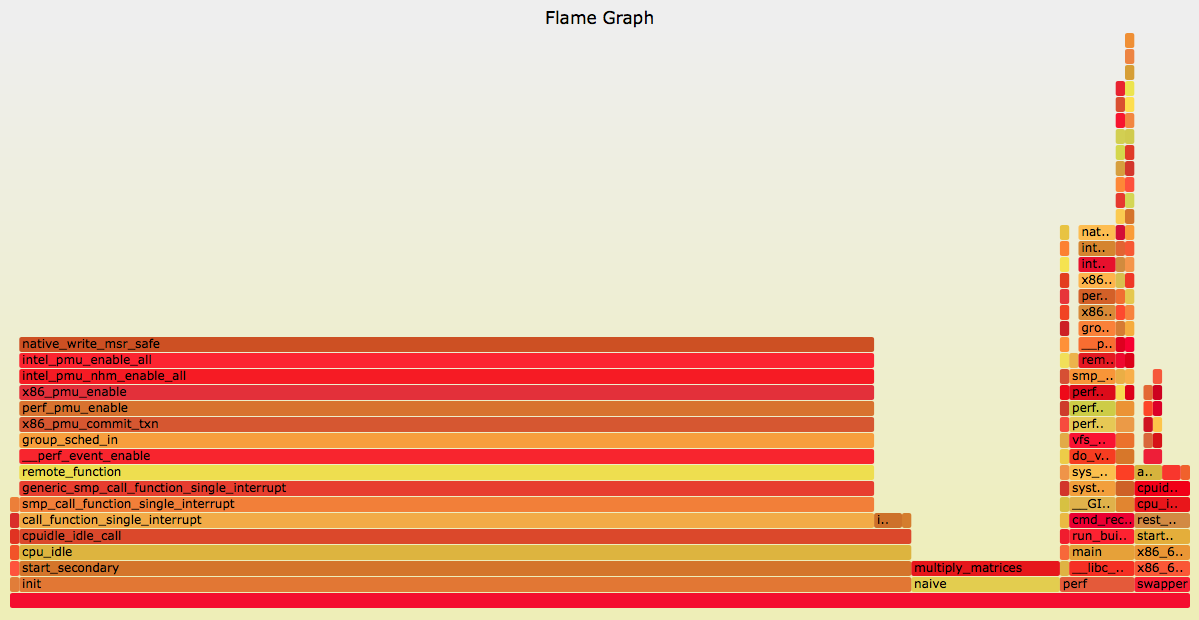
\includegraphics[scale=0.2]{flame_graph_naive.png}
\caption{Flame Graph da Aplicação \textit{naive}}
\end{figure}

\begin{figure}[h!]
\centering
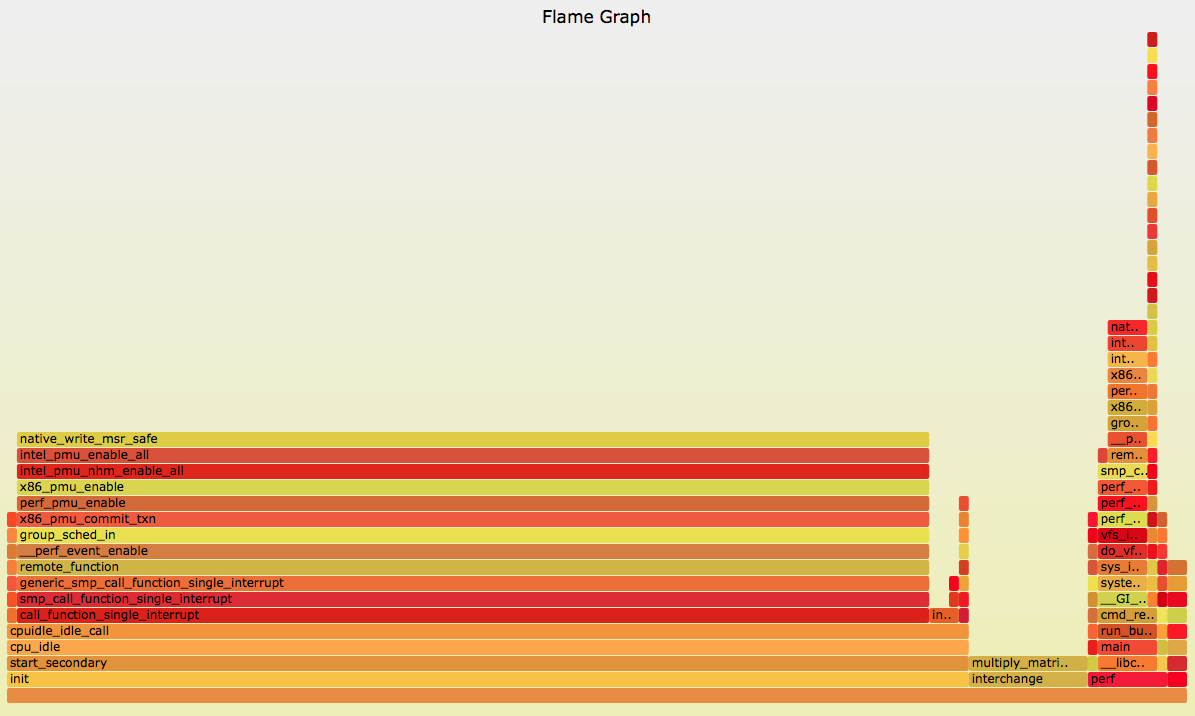
\includegraphics[scale=0.2]{flame_graph_interchange.png}
\caption{Flame Graph da Aplicação \textit{interchange}}
\end{figure}

\begin{figure}[h!]
\centering
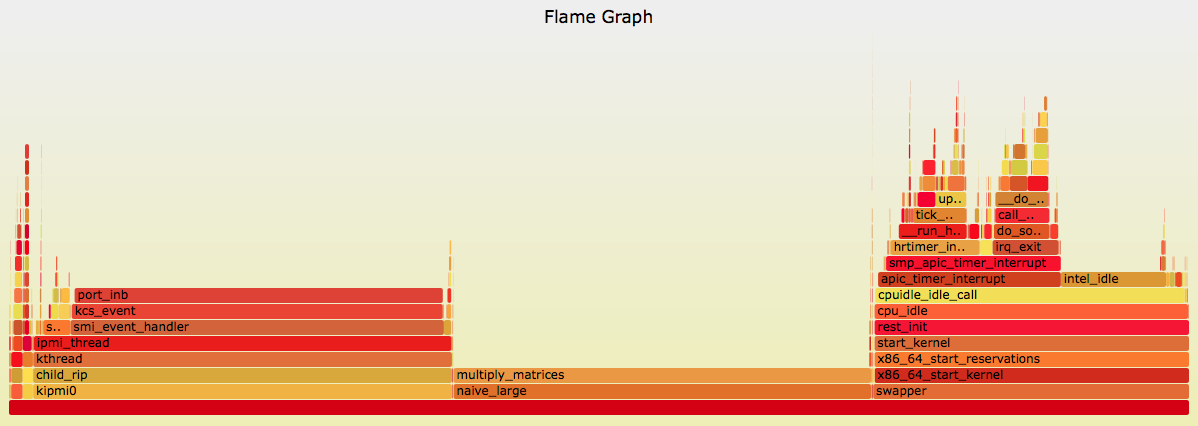
\includegraphics[scale=0.2]{flame_graph_naive_large.png}
\caption{Flame Graph da Aplicação \textit{naive\_large}}
\end{figure}

\begin{figure}[h!]
\centering
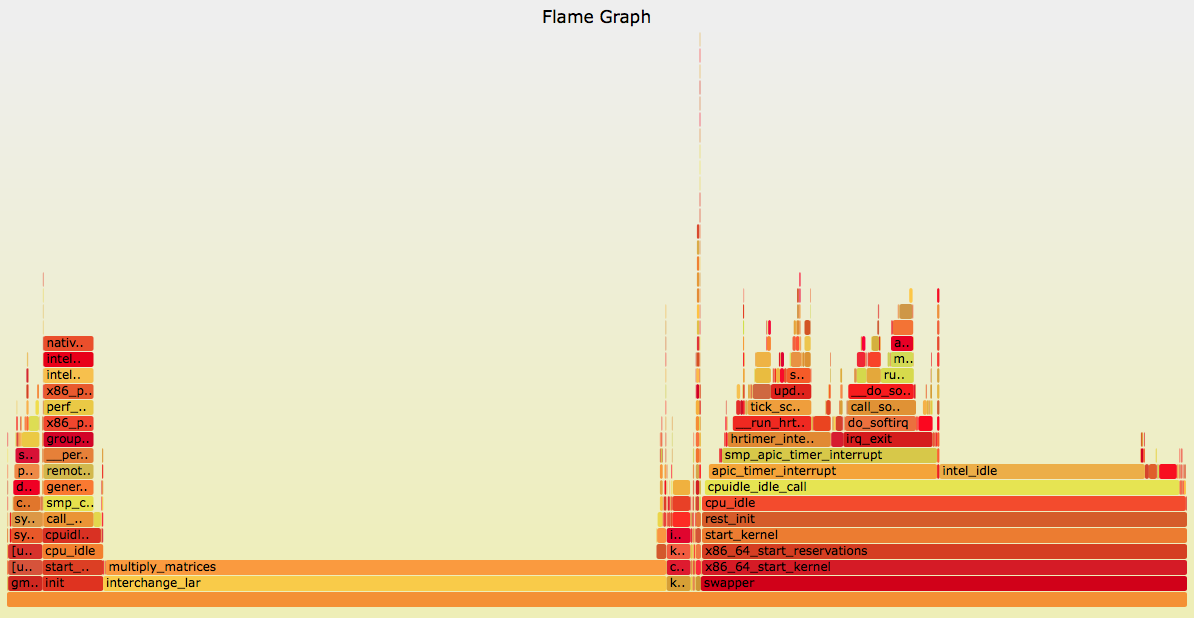
\includegraphics[scale=0.2]{flame_graph_interchange_large.png}
\caption{Flame Graph da Aplicação \textit{interchange\_large}}
\end{figure}

%-----------------------------------
%   Conclusão
%-----------------------------------

\section{Conclusão}
Como foi referido anteriormente, o desenvolvimento deste trabalho tinha como objetivo introduzirmos a ferramenta \textit{perf} e praticarmos a sua utilização. Para isso seguimos o tutorial fornecido pelo professor, tutorial esse que estava dividido em 3 partes. Ao longo destas 3 partes o tutorial sugeria-nos comandos do \textit{perf} para utilizarmos e experimentarmos, graças a este tutorial posso dizer que já tenho um certo conhecimento acerca da utilização da ferramenta \textit{perf}.

Na primeira, deste trabalho foi-nos introduzido o \textit{perf}, apresentando-nos alguns comandos básicos da ferramenta para recolha de informação e leitura/tratamento da mesma, bem como nos ajudou a encontrar \textit{hotspots} numa aplicação. Na segunda parte foi-nos apresentados alguns contadores e fizemos analise dos resultados obtidos para esses contadores. Na ultima e terceira parte, fiz uma analise completa de desempenho para eventos de hardware. Em termos de dificuldades encontradas ao longo do desenvolvimento  deste trabalho posso dizer que não foram muitas, ou mesmo quase nenhumas. 

A maior dificuldade por mim sentida, basicamente foi em termos de analise de alguns resultados, contudo penso que com alguma pesquisa e esforço consegui superar essa dificuldade, acabando por analisar os resultados obtidos. 

No que toca à ferramenta \textit{perf}, posso concluir que é uma ferramenta bastante util, que nos permite fazer uma análise pormenorizada de uma aplicação, permitindo-nos encontrar, por exemplo \textit{hotspots}, que posteriormente podem ser optimizados para obtermos um maior desempenho da aplicação. Para além de considerar uma ferramenta bastante util, considero que o \textit{perf} é bastante prático e fácil de usar, características que a tornam ainda mais interessante.

Quanto à parte dos \textit{Flame Graphs}, posso concluir que é uma técnica bastante prática e fácil de usar/obter. Estes gráficos permite-nos visualizar o perfil do \textit{sotfware} em análise, permitindo-nos ver quais os métodos que consomem mais tempo de CPU, o que torna esta técnica interessante para outro tipo de analise de \textit{software}.

Globalmente, faço uma apreciação bastante positiva deste trabalho, penso que os objetivos foram todos cumpridos e o conhecimento adquirido com o desenvolvimento do trabalho também foi o esperado. Em termos de trabalho futuro, posso dizer que a ferrramenta \textit{perf} vai ser uma ferramenta que vou ter em conta sempre que necessitar de analisar algum código, por isso penso que vai ser bastante utilizada da minha parte daqui para a frente.
% An example of a floating figure using the graphicx package.
% Note that \label must occur AFTER (or within) \caption.
% For figures, \caption should occur after the \includegraphics.
% Note that IEEEtran v1.7 and later has special internal code that
% is designed to preserve the operation of \label within \caption
% even when the captionsoff option is in effect. However, because
% of issues like this, it may be the safest practice to put all your
% \label just after \caption rather than within \caption{}.
%
% Reminder: the "draftcls" or "draftclsnofoot", not "draft", class
% option should be used if it is desired that the figures are to be
% displayed while in draft mode.
%
%\begin{figure}[!t]
%\centering
%\includegraphics[width=2.5in]{myfigure}
% where an .eps filename suffix will be assumed under latex, 
% and a .pdf suffix will be assumed for pdflatex; or what has been declared
% via \DeclareGraphicsExtensions.
%\caption{Simulation results for the network.}
%\label{fig_sim}
%\end{figure}

% Note that the IEEE typically puts floats only at the top, even when this
% results in a large percentage of a column being occupied by floats.


% An example of a double column floating figure using two subfigures.
% (The subfig.sty package must be loaded for this to work.)
% The subfigure \label commands are set within each subfloat command,
% and the \label for the overall figure must come after \caption.
% \hfil is used as a separator to get equal spacing.
% Watch out that the combined width of all the subfigures on a 
% line do not exceed the text width or a line break will occur.
%
%\begin{figure*}[!t]
%\centering
%\subfloat[Case I]{\includegraphics[width=2.5in]{box}%
%\label{fig_first_case}}
%\hfil
%\subfloat[Case II]{\includegraphics[width=2.5in]{box}%
%\label{fig_second_case}}
%\caption{Simulation results for the network.}
%\label{fig_sim}
%\end{figure*}
%
% Note that often IEEE papers with subfigures do not employ subfigure
% captions (using the optional argument to \subfloat[]), but instead will
% reference/describe all of them (a), (b), etc., within the main caption.
% Be aware that for subfig.sty to generate the (a), (b), etc., subfigure
% labels, the optional argument to \subfloat must be present. If a
% subcaption is not desired, just leave its contents blank,
% e.g., \subfloat[].


% An example of a floating table. Note that, for IEEE style tables, the
% \caption command should come BEFORE the table and, given that table
% captions serve much like titles, are usually capitalized except for words
% such as a, an, and, as, at, but, by, for, in, nor, of, on, or, the, to
% and up, which are usually not capitalized unless they are the first or
% last word of the caption. Table text will default to \footnotesize as
% the IEEE normally uses this smaller font for tables.
% The \label must come after \caption as always.
%
%\begin{table}[!t]
%% increase table row spacing, adjust to taste
%\renewcommand{\arraystretch}{1.3}
% if using array.sty, it might be a good idea to tweak the value of
% \extrarowheight as needed to properly center the text within the cells
%\caption{An Example of a Table}
%\label{table_example}
%\centering
%% Some packages, such as MDW tools, offer better commands for making tables
%% than the plain LaTeX2e tabular which is used here.
%\begin{tabular}{|c||c|}
%\hline
%One & Two\\
%\hline
%Three & Four\\
%\hline
%\end{tabular}
%\end{table}


% Note that the IEEE does not put floats in the very first column
% - or typically anywhere on the first page for that matter. Also,
% in-text middle ("here") positioning is typically not used, but it
% is allowed and encouraged for Computer Society conferences (but
% not Computer Society journals). Most IEEE journals/conferences use
% top floats exclusively. 
% Note that, LaTeX2e, unlike IEEE journals/conferences, places
% footnotes above bottom floats. This can be corrected via the
% \fnbelowfloat command of the stfloats package.




% trigger a \newpage just before the given reference
% number - used to balance the columns on the last page
% adjust value as needed - may need to be readjusted if
% the document is modified later
%\IEEEtriggeratref{8}
% The "triggered" command can be changed if desired:
%\IEEEtriggercmd{\enlargethispage{-5in}}

% references section

% can use a bibliography generated by BibTeX as a .bbl file
% BibTeX documentation can be easily obtained at:
% http://mirror.ctan.org/biblio/bibtex/contrib/doc/
% The IEEEtran BibTeX style support page is at:
% http://www.michaelshell.org/tex/ieeetran/bibtex/
%\bibliographystyle{IEEEtran}
% argument is your BibTeX string definitions and bibliography database(s)
%\bibliography{IEEEabrv,../bib/paper}
%
% <OR> manually copy in the resultant .bbl file
% set second argument of \begin to the number of references
% (used to reserve space for the reference number labels box)

\bibliographystyle{abbrv}
\bibliography{ref.bib}
% that's all folks
\end{document}


